\subsection{Physics of Photosensors}

The physical possibility of converting light into electrical charge is at the core of so many key processes in today's world - including biological vision itself. Before we dig into the very concepts of human vision and artificial (silicon) photosensors, it's useful to look in some detail at the basic physical phenomenon that enable such processes. Let's have a look at these:

\subsubsection{Photoelectric Effect}

The photoelectric effect \footnote{Most of this explanation is based on the exellent presentation of the topic on Khan Academy: \url{https://www.khanacademy.org/science/physics/quantum-physics/photons/a/photoelectric-effect}.} is the fundamental physical phenomenon underlying pretty much everything we can do with light: from vision and cameras to the photo-voltaic energy generation. Briefly, it is the emission of electrons when electromagnetic radiation, such as light, hits a material. Electrons emitted in this manner are called photoelectrons and are very useful to say the least. 

\begin{figure}[H]
    \centering
    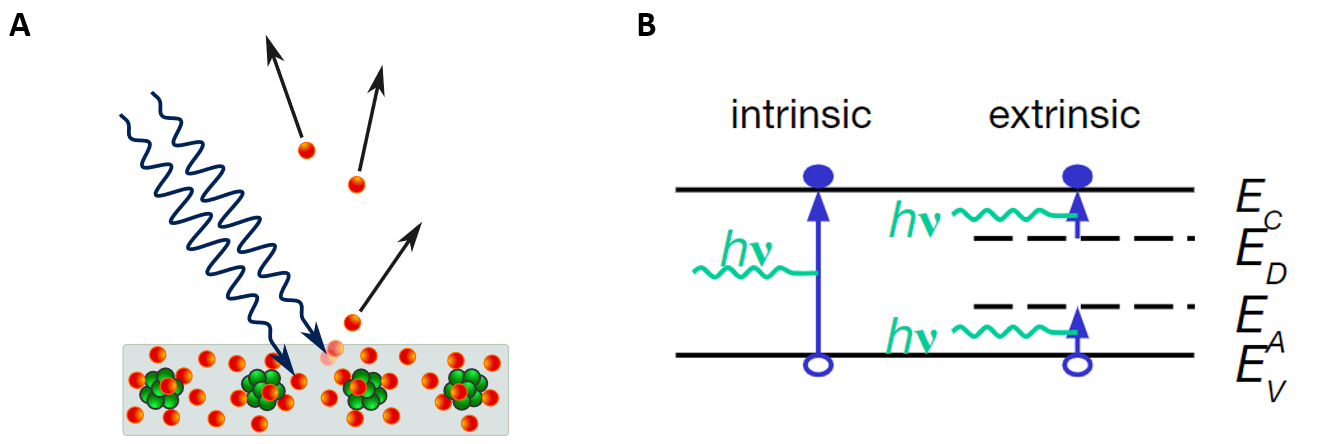
\includegraphics[width=0.9\linewidth]{../../Figures/PhotoElectricEffect.PNG}
    \caption{A) Basic principle of Photoelectric effect. Incident photons represented with the zigzag blue arrows and emittied photoelectrons with the black straight arrows. (Adapted from somewhere on Google Image). B) Photoelectric effect with Band Energy Diagrams applied to Semiconductors. We can see that energy needed for photoelectron emission is higher for intrinsic semiconductor than extrinsic semiconductor. $E_D$ and $E_A$ are Fermi level of N-Type and P-Type semiconductors, respectively. (Adapted from Lecture Notes).}
    \label{fig:PhotoElectricEffect}
\end{figure}

Figure \ref{fig:PhotoElectricEffect}.A) shows the basic intuition behind the photoelectric effect. Incident photons provide some energy that will be enough to take electrons in Valence band out of the valence band and into the conduction band, thus becoming "free" to move! This is best shown in Figure \ref{fig:PhotoElectricEffect}.B). As we established before, the energy of a photon (in vacuum) can be calculated from its wavelength $E_{photon} = h \nu$. 

We can think of the incident light as a stream of photons with a given energy determined by the light frequency. When a photon hits a metal surface, the photon's energy can be \textit{absorbed} by an electron in the metal. This is the same energy principle that we discussed in Chapter 2 when talking about conduction and valence shells, where some energy needed to be brought to free electrons. And exactly as we discussed in chapter 2, there is a minimum energy (so minimum frequency $\v_0$ since energy is determined by frequency) needed to get photoelectrons to be \textit{elevated from valence to conduction band}.  This threshold frequency $\v_0$, you have guessed it, is a property of the material you're projecting photons to, and can best be looked at with energy band diagrams. 

\subsubsection{Optical Absorption}
\subsubsection{Optical Absorption}


Now that we established the basic principes behind photoelectron emission, which comes from absorbtion of photon energy, we should look at some parameters that influence the absorption of photons within a certain material.

When photons are incident onto a surface, they have a certain probability of generating an electron-hole pair, in any "slice" of Silicon. A slice is simply a layer of silicon atoms, that we can also define as an increment depth quantity $\delta x$. As a consequence of this non 0 probability of generating an electron hole pair, the number of photons decreases exponentially within the depth of the surface - the more you go inside the less photos you find because a lot of them have already been absorbed. Every slice $\delta x$ removes some fraction. (See figure \ref{fig:Optical_Absorbtion}.A). This actually varies a lot with wavelength (and thus energy). The longer the wavelength, the lower the energy and the further photons can penetrate before electrons hole pairs are made. This may seem counter-intuitive but it makes sense: it's less likely that low energy (high wavelength) photons create electron hole pairs than higher energy ones - so photons manage to go further inside. This is illustrated in Figure \ref{fig:Optical_Absorbtion}.B). 

\begin{figure}[H]
    \centering
    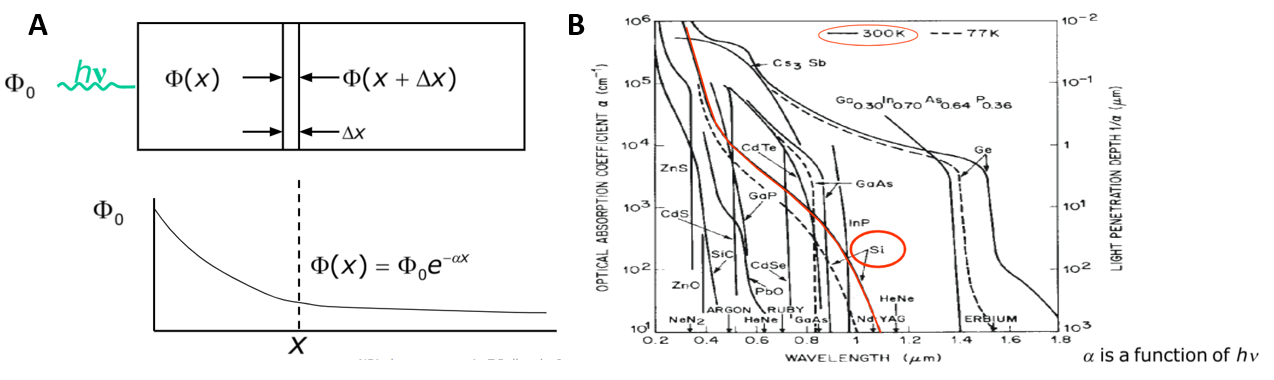
\includegraphics[width=1\linewidth]{../../Figures/Optical_Absorbtion.PNG}
    \caption{A) Schematic of varying photon flux as a function of depth. Top image shows the principle of "Slice" and bottom shows the exponential decay of photons as a function of material depth. B) Absorption as function of wavelength in different material, with Silicon highlighted in red. We can clearly see that optical absorption decreases with increasing wavelength (and thus lower energy). Adapted from Lecture Notes.}
    \label{fig:Optical_Absorbtion}
\end{figure}

Here are the maths underlying the concept. We define photon flux as a function depth $x$ as $\phi(x)$. 
The number of photons absorbed within $\delta x$ is given by the absorption coefficient $alpha$:

\begin{equation}
    \frac{d\phi(x)}{dx} = -\alpha \phi(x)
\end{equation}
This differential equation can easily be solved:
\begin{equation}
    \phi(x) =  \phi_0(x) e^{-\alpha x} 
\end{equation}

The $\phi_0$ propety is important and factor of a few things, such as Reflection $R$, cross section $A$ and incident optical power $P_{opt}$. I mention these only for reference, knowing this is not required for the exam - though this should intuitively make sense. 

\begin{equation}
    \phi_0 = \frac{1-R}{A}\cdot \frac{\lambda}{hc}\cdot P_{opt}
\end{equation}

In silicon, the longest wave length that can create photoelectrons is 1.1 $\mu m$ - just above visible domain. Huh, once again, we're in luck, Silicon happens to have just what we need. 


\subsubsection{Quantum Efficiency}

One last thing to talk about before we start looking at the details of some actual sensors: quantum efficiency. Quantum efficiency, $\eta$ (or $QE$) is defined as the number of electron-hole pairs generated for each incident photon (always $<=1$ !!). This is particularly important to evaluate the quality of photosensors, and also is a very important measure for solar energy things. Of course you want a high number of electrons (and thus current) to be emitted from light. This is really what needs to be optimized in a photosensor. This concept should become clearer when talking about specific photosensors, so hold it if it's not clear yet. 

\begin{equation}
    \eta = \frac{I_{ph}}{q}\cdot \frac{hc/\lambda}{P_{opt}}
\end{equation}

With $I_{ph}$ photogenerated current, $q$ number of carriers (electron or holes) and $P_{opt}$ incident optical power.

\begin{figure}[H]
    \centering
    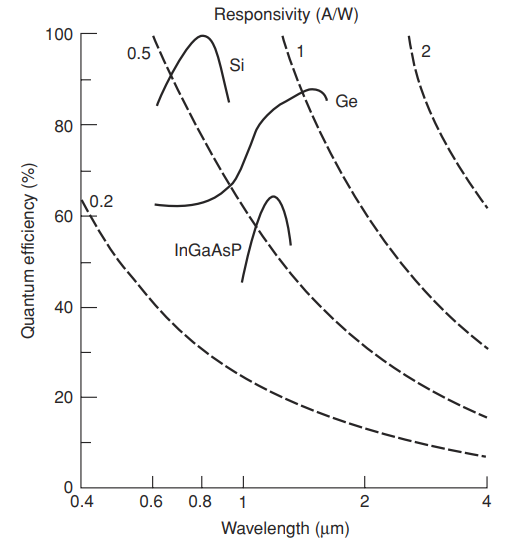
\includegraphics[width=0.6\linewidth]{../../Figures/Quantum_Efficiency.PNG}
    \caption{Quantum efficiencies and responsivities of photosensors fabricated from different semiconductors. Silicon exhibits a very good quantum efficiency peaking in the near infrared which may approach 100\% in a certain spectral range. Adapted from Textbook.}
    \label{fig:Quantum_Efficiency}
\end{figure}




